\documentclass{scrreprt}
\usepackage{listings}
\usepackage{underscore}
\usepackage{graphicx}
\usepackage[bookmarks=true]{hyperref}
\usepackage[utf8]{inputenc}
\usepackage[german]{babel}
\hypersetup{
    bookmarks=false,    % show bookmarks bar?
    pdftitle={Software Requirement Specification},    % title
    pdfauthor={Fischer, Tobias \\
Libak, Miklós \\
Norkunas, Eva \\
Weinknecht, Lucas \\},                     % author
    pdfsubject={TeX and LaTeX},                        % subject of the document
    pdfkeywords={TeX, LaTeX, graphics, images}, % list of keywords
    colorlinks=true,       % false: boxed links; true: colored links
    linkcolor=blue,       % color of internal links
    citecolor=black,       % color of links to bibliography
    filecolor=black,        % color of file links
    urlcolor=purple,        % color of external links
    linktoc=page            % only page is linked
}%
\def\myversion{0.1 }
\date{}
%\title
\usepackage{hyperref}
\begin{document}

\begin{flushright}
    \rule{16cm}{5pt}\vskip1cm
    \begin{bfseries}
        \Huge{SOFTWARE REQUIREMENTS\\ SPECIFICATION}\\
        \vspace{1.5cm}
        for\\
        \vspace{1.5cm}
        MELT Chess\\
        \vspace{1.5cm}
        \LARGE{Version \myversion}\\
        \vspace{1.5cm}
        \vspace{1.5cm}
        \today\\
    \end{bfseries}
\end{flushright}

\tableofcontents

\chapter{Einführung}

\section{Projektanforderungen}
Entwickelt werden soll ein Schach Programm, welches es ermöglicht gegeneinander als auch gegen eine künstliche Intelligenz Schach zu spielen. Das Spiel soll dafür sowohl über eine graphische als auch über eine konsolenbasierte Benutzerschnittstelle verfügen. Das Spiel soll in englischer Sprache umgesetzt werden. Die Entwicklung soll sich dabei in drei Iterationen gliedern. In diesem Dokument sind die Anforderungen an die erste Iteration dargelegt.

\section{Zielgruppe des Dokuments und weitere Resourcen}
Dieses Anforderungsdokument richtet sich zum einen an die beteiligten Entwickler und dient zur Orientierung ob die Funktionalität des Projekt gemäß den Anforderungen umgesetzt wird, und zum anderen an die Kontaktperson(en) des Moduls um die Planung des Projekts zu überprüfen.

Einen weiteren Überblick bieten die Storycards, welche im Gitlab des Projekts zu finden sind und in Form von Issues umgesetzt werden.

\chapter{Umfang des Projekts}
\section{Funktionale Anforderungen}
Zum Umfang gehört in der 1. Iteration des Projekts die Bereitstellung einer Textbasierten Konsolen-Schnittstelle in der es möglich ist Mensch-gegen-Mensch Spiele zu spielen. Dazu ist die Umsetzung des Pakets model nötig, in dem der Zustand des Bretts sowie die Schachregeln\footnote{Nach den Regeln des Weltschachverbands (FIDE) in der deutschen Übersetzung von 2018} implementiert werden.

In der 2. Iteration wird die geschaffene Basis durch eine 2D-GUI unter Verwendung des JavaFX Moduls erweitert und eine rudimentäre Schach KI im Modul engine erstellt.

In der 3. Iteration soll die Anwendung um Netzwerkfähigkeit mit der Anwendung der Gruppe 2 erweitert werden. Zusätzlich soll eine Auswahl von möglichen Erweiterungen umgesetzt werden, welche in Summe einen Aufwand von mindestens 10 Einheiten aufweisen müssen. Die Auswahl mit möglicher Punktzahl lauten:

\begin{itemize}
\item Verbesserte KI mithilfe Min-/Max-Suche mit $\alpha$/$\beta$-Pruning (5)
\item 3D-GUI (5)
\item Eindimensionales Schach (5)
\item Rückgängig-Machen von Zügen (3)
\item Speichern/Laden von Spielen (3)
\item Schachuhren (2)
\item Zweisprachigkeit (2)
\item Resizeable GUI (1)
\end{itemize}

\section{Nicht-funktionale Anforderungen}

\subsection{Codingstyle, Metriken, Testabdeckung}
Das Template verwendet die Plugins PMD und JaCoCo zur Generierung von Reports über Metriken, Codestyle und Testabdeckung.
Es wird eine Testabdeckung des gesamten Codes von 90\% Instruction Coverage erwartet, ausgenommen der GUI-Klassen.
Im Template wird ein PMD-Regelsatz eingebunden. Diese Regeln sind für den Code und die Testfälle einzuhalten.


\subsection{Überprüfungen}
Es soll mindestens alle zwei Wochen ein Treffen mit dem zugewiesenen Tutor stattfinden. Neben den Deadlines der drei Iterationen gibt es außerdem noch folgende Termine:

\begin{itemize}
\item 23.04.2021: Abgabe Anforderungsanalyse, Vorgehensplan, Prüfung erfolgreiche Einrichtung der Infrastruktur

\item 19.05.2021: Prüfung, ob auslieferbare Version vorliegt, die Anforderungen der ersten Iteration genügt mit automatisierten Tests und Theorie-Abfrage

\item 16.06.2021: Prüfung, ob auslieferbare Version vorliegt, die
Anforderungen der zweiten Iteration genügt mit Zwischenpräsentation

\item 14.07.2021: Endabgabe mit Abschlusspräsentation
\end{itemize}

\subsection{Abgabeformat}
An den Schlusstagen der Iterationen, inklusive Endabgabe, muss der zu überprüfende/bewertende Stand mittels Tags (it1,it2,...) im git-Repository gekennzeichnet werden.

\chapter{Anhang}
\section{Tabellarische Anforderungsanalyse}
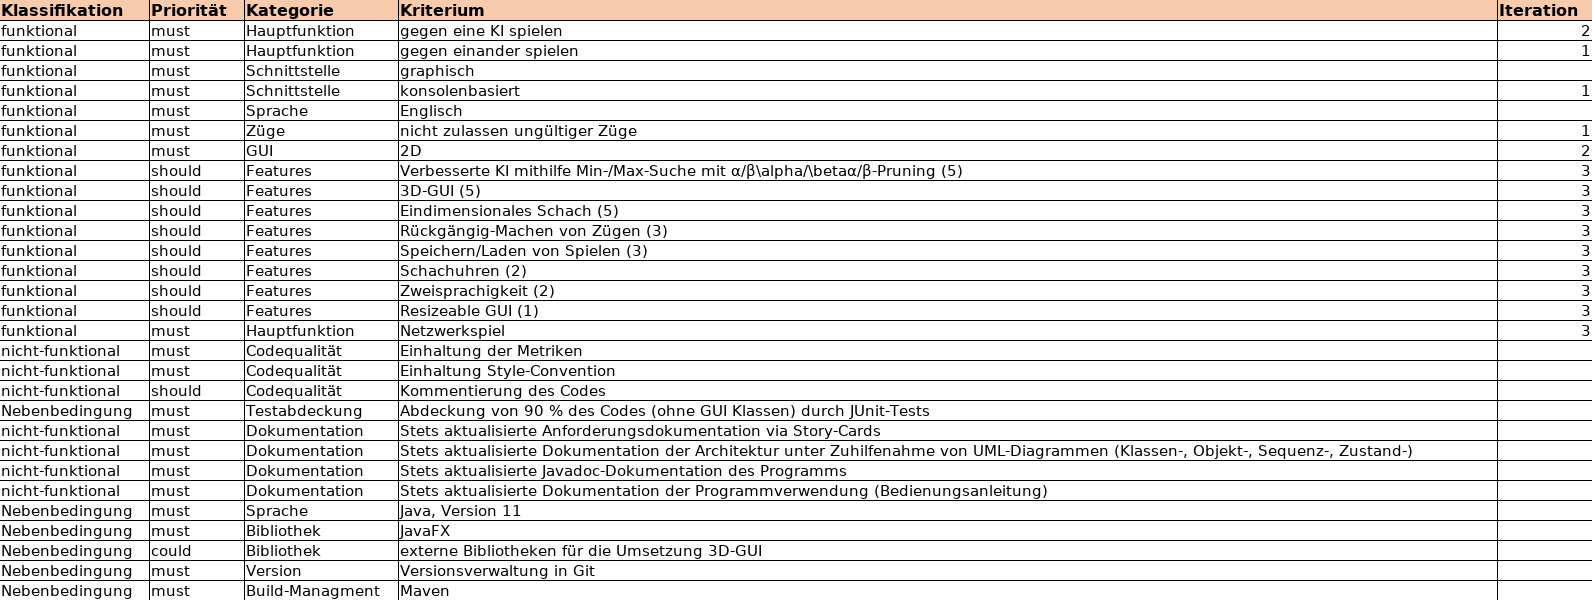
\includegraphics{resources/anforderungsanalyse_tabelle.png}
\end{document}
